\documentclass[pdf,mia,noFooter,slideColor,colorBG]{prosper}

\usepackage{amsmath, amssymb}
\usepackage{epsfig}
\usepackage{color}

\definecolor{orange}{rgb}{.98,.3,.03}
\newcommand{\emphase}[1]{{\textcolor{blue}{{#1}}}}
\newcommand{\orange}[1]{{\textcolor{orange}{{#1}}}}
\renewcommand{\paragraph}[1]{{\large \bf  #1}}


%====================================
\begin{document}
%====================================

%====================================
\begin{slide}{}
  \psline[linewidth=50pt,linecolor=white](-2,1.4)(10.3,1.4)
  \rput[lb](2.5cm,0.4cm){\includegraphics[width=5cm]{Page1_top.eps}}
  \rput[lb](-0.3cm,-1.4cm){\includegraphics[width=10.5cm]{logoMIA19x2.eps}}
  \rput[lb](0.8cm,-4.8cm){Evaluation of the MIA Department -- October 2006}
  \rput[lb](-1.8cm,-5.2cm){\rotatebox[origin=c]{0}{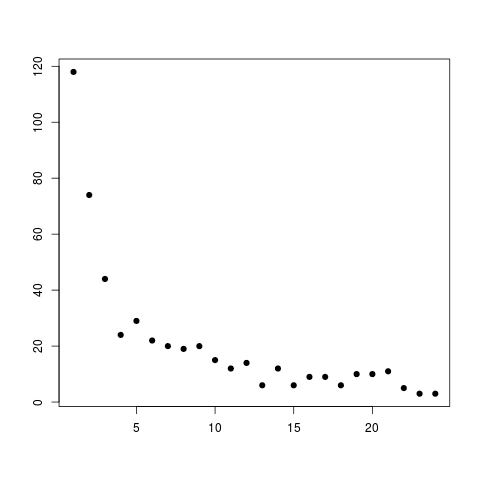
\includegraphics[width=2cm]{butterfly.eps}}} 
  \rput[lb](-2cm,-7.35cm){\includegraphics[width=13.7cm]{Page1_bottom.eps}}
 
  \rput[lb](0.5cm,-2.1cm){\large\textbf{\orange{S}tatistics for \orange{S}ystems \orange{B}iology}}
\end{slide}
%====================================

%====================================
\begin{slide}{SSB group}
\begin{itemize}
\item 24 scientists (+ 6 PhD).
\item 3 MIA units: Evry, Jouy (MIG), Paris.
\item Existence from 10 years.
\item Strong interactions.
\item Regular meetings (1 day per month).
\item \url{www.genome.jouy.inra.fr/ssb/}
\end{itemize}

% MIG : SS, FR, PN, CH, [ER, AG]

% Evry : BP, FM, AST, GN, CM, EB, MH, VM, CC, CA [FP, SL, MG]

% Paris : SR, JJD, EL, TMH, JA, MLM, AB, NC, [MM, AC, MK]
\end{slide}
%====================================

%====================================
\overlays{2}{%
\begin{slide}{3 Major Research fields}
\vspace{0.5cm}
\begin{description}
\item[\paragraph{Sequence analysis:}] ~\\
  \emphase{Motifs} (discrete
  math., large deviation, Poisson approximation, scan statistics). \\
  \emphase{Local and alignment scores} (CUSUM processes, random walks,
  paired HMM). \\
\onlySlide*{1}{
\emphase{Gene, motif and 2D structure prediction} (HMM,
  semi-Markov hidden models).
}
\onlySlide{2}{
\orange{Gene, motif and 2D structure prediction} (HMM,
  semi-Markov hidden models).
}
\end{description}
\end{slide}
}
%====================================

%====================================
\overlays{3}{%
\begin{slide}{}%3 Major Research Fields (2)}
\vspace{-0.75cm}
\begin{description}
\FromSlide{1}
\item[\paragraph{Microarray data:}] ~\\
  \emphase{Experimental design} (linear model). \\ 
  \emphase{Differential analysis} (multiple testing, mixture model). \\
  \emphase{Diagnostic} (supervised classification, dimension reduction, model
  selection). \\ 
  \emphase{Comparative Genomic Hybridisation} (breakpoint
  detection, mixed model).\\
  ~\\
\FromSlide{2}
\item[\paragraph{Biological networks:}] ~\\
\onlySlide*{2}{  
  \emphase{Random graph models}
  (mixture models, variational methods, discrete math.). \\
  \emphase{Motifs} (Combinatorics, Poisson approximation). 
}
\onlySlide*{3}{
 \orange{Random graph models}
  (mixture models, variational methods, discrete math.). \\
  \orange{Motifs} (Combinatorics, Poisson approximation).
}
  \emphase{Network inference} (Graphical models, multiple testing).
\end{description}
\end{slide}
}
%====================================

\begin{slide}{Sequence Analysis via HMM}
\end{slide}
%====================================



\end{document}